\documentclass{article}

<<<<<<< HEAD

%For 3D plots
\usepackage{blindtext}
\usepackage{pgfplots}
\pgfplotsset{compat=1.9}
% For inline color changes
\usepackage{xcolor}
=======
>>>>>>> c733b4c556979a7348397865067ed20806b6465e
% For vertical brace rcases
\usepackage{mathtools}
% For positioning figures
\usepackage{float}
% makes figure font bold
\usepackage{caption}
\captionsetup[figure]{labelfont=bf}
% For text generation
\usepackage{lipsum}
% For drawing
\usepackage{tikz}
% For manipulating coordinates
\usetikzlibrary{calc}
% For relative node positioning
\usetikzlibrary{positioning}
% For smaller or equal sign and not divide sign
\usepackage{amssymb}
% For the diagonal fraction
\usepackage{xfrac}
% For enumerating exercise parts with letters instead of numbers
\usepackage{enumitem}
% For dfrac, which forces the fraction to be in display mode (large) e
% even in math mode (small)
\usepackage{amsmath}
% For degree sign
\usepackage{gensymb}
% For "\mathbb" macro
\usepackage{amsfonts}
\newcommand{\N}{\mathbb{N}}
\newcommand{\Z}{\mathbb{Z}}
\newcommand{\Q}{\mathbb{Q}}
\newcommand{\R}{\mathbb{R}}
\newcommand{\C}{\mathbb{C}}
\newcommand{\F}{\mathbb{F}}
\newcommand{\rad}{\text{ rad}}
\newcommand{\lcm}{\text{lcm}}
\newcommand{\Aut}{\text{Aut}}
\newcommand{\seq}{\leqslant}
\newcommand{\beq}{\geqslant}
\newcommand{\sub}{\subseteq}
\newcommand{\prosub}{\subset}

\newcommand{\Ocal}{\mathcal{O}}
\newcommand{\Ccal}{\mathcal{C}}
\newcommand{\Pcal}{\mathcal{P}}
\newcommand{\Scal}{\mathcal{S}}

% overline short italic
\newcommand{\olsi}[1]{\,\overline{\!{#1}}}

\title{%
    \Huge Abstract Algebra \\
    \large by \\
    \Large Dummit and Foote \\~\\
    \huge Part 1: Group Theory \\
    \LARGE Chapter 2: Subgroups \\
    \Large Section 5: The Lattice of Subgroups of a Group
}
\date{2023-07-14}
\author{Michael Saba}

\begin{document}
    \pagenumbering{gobble}
    \maketitle
    \newpage
    \pagenumbering{arabic}


    \section*{Exercise 1}
    For $\{1\} \seq H, K \seq G$,
    (there can be other subgroups)
    the possible sublattices of $G$ containing only these groups are:

    \begin{figure}[H]
        \centering
        % figure is a tikz drawing
        \begin{tikzpicture}[scale=2.5]

        \def\d{.7cm}

        % Specifies where the x, y coordinate of the tip of
        % the unite vectors in turn
        \tikzset{}
        
        % Scope used to shift the coordinates from the basis
        \begin{scope}[shift={(0, 0, 0)}, rotate=0]
            \node (G1) at (0, 0) {$G$};   
            \node (H1) [below left=\d and \d of G1] {$H$};   
            \node (K1) [below right=\d and \d of G1] {$K$};   
            \node (T1) [below right=\d and \d of H1] {$\left\{ 1 \right\}$}; 
            
            \node (G2) at (2, 0) {$G$};   
            \node (H2) [below left=\d and \d of G2] {$H$};   
            \node (K2) [below left=\d and \d of H2] {$K$};   
            \node (T2) [below left=\d and \d of K2] {$\left\{ 1 \right\}$}; 

            \node (G3) at (3, 0) {$G$};   
            \node (K3) [below left=\d and \d of G3] {$K$};   
            \node (H3) [below left=\d and \d of K3] {$H$};   
            \node (T3) [below left=\d and \d of H3] {$\left\{ 1 \right\}$}; 
        \end{scope}

        \begin{scope}[thick]
            \draw (G1) -- (H1);
            \draw (G1) -- (K1);
            \draw (K1) -- (T1);
            \draw (H1) -- (T1);

            \draw (G2) -- (H2);
            \draw (H2) -- (K2);
            \draw (K2) -- (T2);

            \draw (G3) -- (K3);
            \draw (K3) -- (H3);
            \draw (H3) -- (T3);
        \end{scope} 

        \end{tikzpicture}

        \caption{\label{fig:figure1} Possible sublattices of the group $G$.}
    \end{figure} 

    The sublattices are distinguished by the inclusions
    of $H$ and $K$. While it's always the case that $\{1\}$
    is contained in all subgroups and $G$ contains all subgroups,
    $H$ and $K$ can contain one another or not.


    \section*{Exercise 2}
    Going by the lattice of $D_{16}$: 

    \begin{figure}[H]
        \centering
        % figure is a tikz drawing
        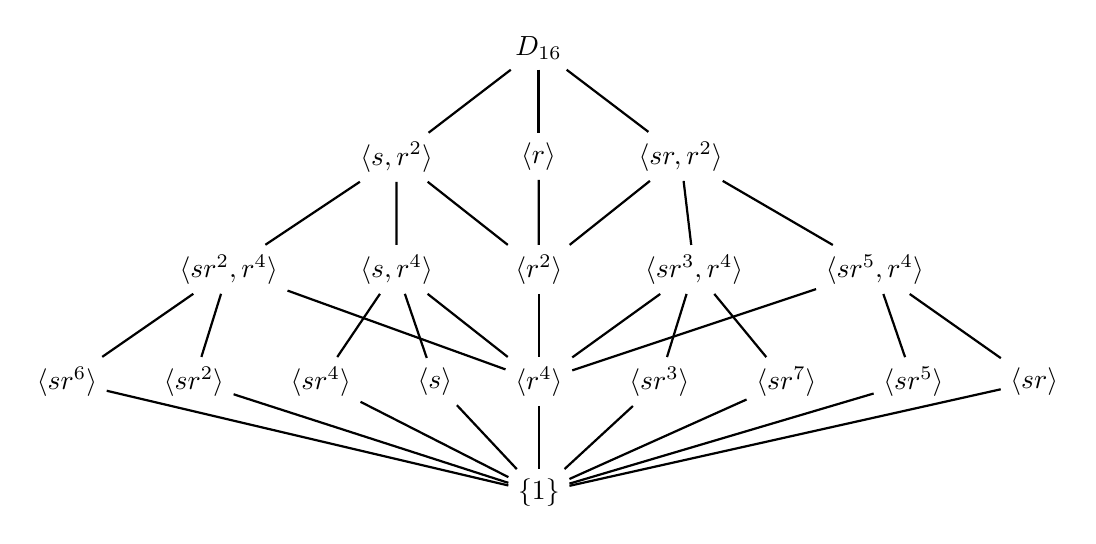
\begin{tikzpicture}[scale=2.5]

        \def\d{.8cm}
        \def\h{.6cm}

        % Specifies where the x, y coordinate of the tip of
        % the unite vectors in turn
        \tikzset{}
        
        % Scope used to shift the coordinates from the basis
        \begin{scope}[shift={(0, 0, 0)}, rotate=0]
            \node (D16) at (0, 0) {$D_{16}$};   
            \node (A1) [below left=\d and \d of D16]
            {$\langle s, r^2 \rangle$}; 
            \node (A2) [below= \d of D16] {$\langle r \rangle$}; 
            \node (A3) [right= \d of A2]
            {$\langle sr, r^2 \rangle$};  
            \node (B1) [below left=\d and \d of A1]
            {$\langle sr^2, r^4 \rangle$}; 
            \node (B2) [right=\d of B1] {$\langle s, r^4 \rangle$}; 
            \node (B3) [right=\d of B2]
            {$\langle r^2 \rangle$};  
            \node (B4) [right=\d of B3] {$\langle sr^3, r^4 \rangle$}; 
            \node (B5) [right=\d of B4]
            {$\langle sr^5, r^4 \rangle$};  

            \node (C1) [below left=\d and \d of B1]
            {$\langle sr^6 \rangle$}; 
            \node (C2) [right= \h of C1]
            {$\langle sr^2 \rangle$}; 
            \node (C3) [right= \h  of C2]
            {$\langle sr^4 \rangle$}; 
            \node (C4) [right= \h of C3]
            {$\langle s \rangle$}; 
            \node (C5) [below= \d of B3] {$\langle r^4 \rangle$};
            \node (C6) [right= \h of C5]
            {$\langle sr^3 \rangle$}; 
            \node (C7) [right= \h of C6]
            {$\langle sr^7 \rangle$};
            \node (C8) [right= \h of C7]
            {$\langle sr^5 \rangle$};  
            \node (C9) [right= \h of C8]
            {$\langle sr \rangle$};  
            
            \node (T1) [below=\d of C5] {$\left\{ 1 \right\}$}; 
        \end{scope}

        \begin{scope}[thick]
            \draw (D16) -- (A1);
            \draw (D16) -- (A2);
            \draw (D16) -- (A3);
            \draw (A1) -- (B1);
            \draw (A1) -- (B2);
            \draw (A1) -- (B3);
            \draw (A3) -- (B5);
            \draw (A3) -- (B4);
            \draw (A3) -- (B3);
            \draw (A2) -- (B3);
            \draw (B3) -- (C5);
            \draw (B1) -- (C1);
            \draw (B1) -- (C2);
            \draw (B1) -- (C5);
            \draw (B2) -- (C3);
            \draw (B2) -- (C4);
            \draw (B2) -- (C5);
            \draw (B4) -- (C6);
            \draw (B4) -- (C7);
            \draw (B4) -- (C5);
            \draw (B5) -- (C8);
            \draw (B5) -- (C9);
            \draw (B5) -- (C5);

            \foreach\x in {1,..., 9}
            \draw (C\x) -- (T1);
        \end{scope} 

        \end{tikzpicture}

        \caption{\label{fig:figure1} Lattice of $D_{16}.$}
    \end{figure} 

    \begin{enumerate}[label=\textbf{\alph*.}]
        \item 
            We have \[ \langle sr^2, r^4 \rangle
            \beq \langle sr^2, r^4 \rangle, \langle sr^6 \rangle,
            \langle sr^2 \rangle, \langle r^4 \rangle, \{1\} \]
        \item 
            We have \[ \langle sr^7, r^4 \rangle = \langle sr^3, r^4 \rangle 
            \beq \langle sr^3, r^4 \rangle, \langle sr^3 \rangle,
            \langle sr^7 \rangle, \langle r^4 \rangle, \{1\} \]
        \item 
            We have         
            \begin{align*}
                \langle r^4 \rangle
                \seq \langle r^4 \rangle, \langle sr^2, r^4 \rangle,
                \langle s, r^4 \rangle, \langle sr^3, r^4 \rangle,
                \langle sr^5, r^4 \rangle, \langle r^2 \rangle,
                \langle r \rangle, \langle s, r^2 \rangle, \\
                \langle sr, r^2 \rangle, \langle r \rangle, D_{16}
            \end{align*}
        \item 
            We have \[ \langle s \rangle
            \seq  \langle s \rangle, \langle s, r^4 \rangle,
            \langle s, r^2 \rangle, D_{16} \]
    \end{enumerate}


    \section*{Exercise 3}
    Proof that in $D_8$, $\langle s, r^2 \rangle \cong V_4$
    (\textit{the Klein Group}): \\
    We can probe that $\langle s, r^2 \rangle \cong V_4$
    by drawing their group tables:

    \begin{figure}[H]
        \centering

        \[\vbox{\tabskip0.5em\offinterlineskip
        \halign{\strut$#$\hfil\ \tabskip1em\vrule&&$#$\hfil\cr
        ~   & 1   & a   & b & c \cr
        \noalign{\hrule}\vrule height 12pt width 0pt
        1   & 1 & a & b & c \cr 
        a   & a & 1 & c & b \cr 
        b   & b & c & 1 & a \cr 
        c   & c & b & a & 1 \cr
        }}\]

        
        \[\vbox{\tabskip0.5em\offinterlineskip
        \halign{\strut$#$\hfil\ \tabskip1em\vrule&&$#$\hfil\cr
        ~   & 1   & s   & r^2 & sr^2 \cr
        \noalign{\hrule}\vrule height 12pt width 0pt
        1   & 1 & s & r^2 & sr^2 \cr 
        s   & s & 1 & sr^2 & r^2 \cr 
        r^2   & r^2 & sr^2 & 1 & s \cr 
        sr^2   & sr^2 & r^2 & s & 1 \cr
        }}\]

        \caption{\label{fig:figure1} The group tables of $V_4$
        and $\langle s, r^2 \rangle$.}
    \end{figure}

    By mapping $a$ to $s$, $b$ to $r^2$, and $c$ to $sr^2$,
    the tables are equivalent,
    so the groups are isomorphic. \\ 
    Alternatively, we can refer to a later proof in exercise 1.2.5.10
    which states that there are only two unique groups of order 4,
    the cyclic group $Z_4 = \langle x \rangle$,
    and the non-cyclic Klein Group $V_4 = \{1, a, b, c\}$.
    This means that $\langle s, r^2 \rangle$
    is isomorphic to one of them.
    Since it is by deifnition not generated by a single element,
    it can't be isomorphic to $Z_4$,
    so it is isomorphic to $V_4$.


    \section*{Exercise 4}
    We know that $D_8$ is generated by $r$ and $s$,
    so $D_8 = \langle r, s \rangle$.
    So we need to look at the lattice of $D_8$
    and count all the pairs of elements that aren't equal to 
    any of the proper subgroups of $D_8$.
    If for instance, $\langle x, y \rangle$ where $x, y \in D_8$
    isn't a proper subgroup of $D_8$,
    then, since $D_8$ is closed under inverses and composition,
    this can only mean that $D_8 = \langle x, y \rangle$.
    So, given

    \begin{figure}[H]
        \centering
        % figure is a tikz drawing
        \begin{tikzpicture}[scale=2.5]

        \def\d{.8cm}

        % Specifies where the x, y coordinate of the tip of
        % the unite vectors in turn
        \tikzset{}
        
        % Scope used to shift the coordinates from the basis
        \begin{scope}[shift={(0, 0, 0)}, rotate=0]
            \node (Q8) at (0, 0) {$D_8$};   
            \node (A1) [below left=\d and \d of G1]
            {$\langle s, r^2 \rangle$}; 
            \node (A2) [below= \d of G1] {$\langle r \rangle$}; 
            \node (A3) [below right=\d and \d of G1]
            {$\langle rs, r^2 \rangle$};  
            \node (B1) [below left=\d and \d of A1]
            {$\langle r^2s \rangle$}; 
<<<<<<< HEAD
            \node (B2) [below= \d of A1] {$\langle s \rangle$}; 
=======
            \node (B2) [below= \d of A1] {$\langle r^2s \rangle$}; 
>>>>>>> c733b4c556979a7348397865067ed20806b6465e
            \node (B3) [below=\d of A2]
            {$\langle r^2 \rangle$};  
            \node (B4) [below= \d of A3] {$\langle rs \rangle$}; 
            \node (B5) [below right=\d and \d of A3]
            {$\langle r^3s \rangle$};  
            \node (T1) [below=\d of B3] {$\left\{ 1 \right\}$}; 
        \end{scope}

        \begin{scope}[thick]
            \draw (Q8) -- (A1);
            \draw (Q8) -- (A2);
            \draw (Q8) -- (A3);
            \draw (A1) -- (B1);
            \draw (A1) -- (B2);
            \draw (A1) -- (B3);
            \draw (A3) -- (B5);
            \draw (A3) -- (B4);
            \draw (A3) -- (B3);
            \draw (A2) -- (B3);

            \foreach\x in {1,..., 5}
            \draw (B\x) -- (T1);
        \end{scope} 

        \end{tikzpicture}

        \caption{\label{fig:figure1} Lattice of $D_8.$}
    \end{figure} 

    With that, we have that
    $\langle r, s \rangle$, $\langle r^3, s \rangle$,
    $\langle sr, s \rangle$, $\langle sr^3, s \rangle$,
    $\langle r^3, sr \rangle$, $\langle r^3, sr^3 \rangle$,
    $\langle sr, sr^3 \rangle$, $\langle sr, r \rangle$,
    $\langle sr, r^3 \rangle$, $\langle sr, sr^2 \rangle$,
    $\langle sr^2, r \rangle$, $\langle sr^3, r \rangle$
    are all 12 of the unique pairs of elements that 
    generate all of $D_8$
    instead of being equal to one of its proper subgroups.


    \section*{Exercise 5}
    We need to find all 8 elements $x \in D_{16}$
    such that $\langle x, s \rangle = D_{16}$.
    Like exercise 1.2.5.4, we can do this by finding
    all values of $x$ for which the group $\langle x, s \rangle$
    is not equal to one of the subgroups of $D_{16}$ in its lattice

    \begin{figure}[H]
        \centering
        % figure is a tikz drawing
        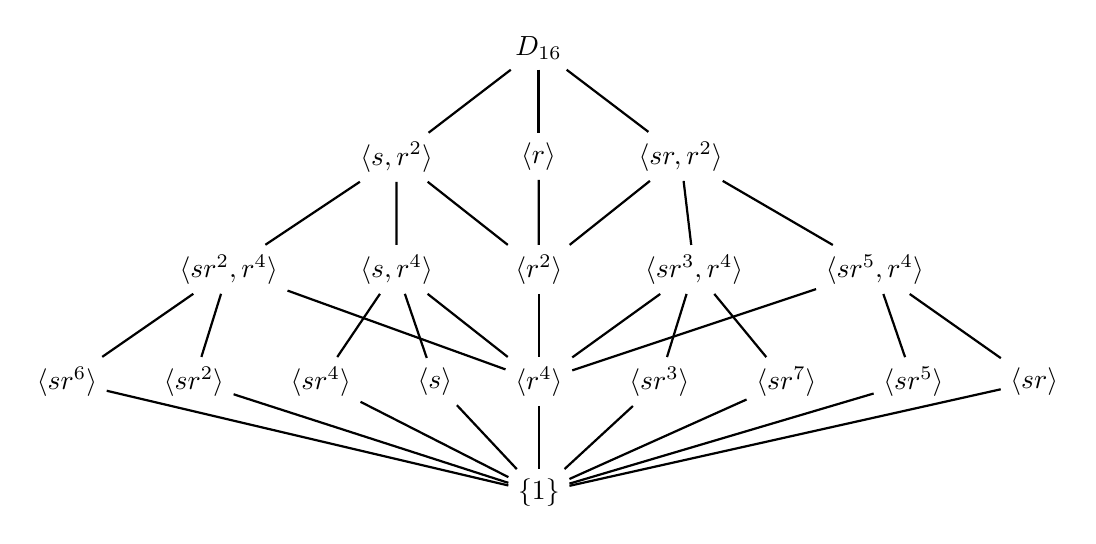
\begin{tikzpicture}[scale=2.5]

        \def\d{.8cm}
        \def\h{.6cm}

        % Specifies where the x, y coordinate of the tip of
        % the unite vectors in turn
        \tikzset{}
        
        % Scope used to shift the coordinates from the basis
        \begin{scope}[shift={(0, 0, 0)}, rotate=0]
            \node (D16) at (0, 0) {$D_{16}$};   
            \node (A1) [below left=\d and \d of D16]
            {$\langle s, r^2 \rangle$}; 
            \node (A2) [below= \d of D16] {$\langle r \rangle$}; 
            \node (A3) [right= \d of A2]
            {$\langle sr, r^2 \rangle$};  
            \node (B1) [below left=\d and \d of A1]
            {$\langle sr^2, r^4 \rangle$}; 
            \node (B2) [right=\d of B1] {$\langle s, r^4 \rangle$}; 
            \node (B3) [right=\d of B2]
            {$\langle r^2 \rangle$};  
            \node (B4) [right=\d of B3] {$\langle sr^3, r^4 \rangle$}; 
            \node (B5) [right=\d of B4]
            {$\langle sr^5, r^4 \rangle$};  

            \node (C1) [below left=\d and \d of B1]
            {$\langle sr^6 \rangle$}; 
            \node (C2) [right= \h of C1]
            {$\langle sr^2 \rangle$}; 
            \node (C3) [right= \h  of C2]
            {$\langle sr^4 \rangle$}; 
            \node (C4) [right= \h of C3]
            {$\langle s \rangle$}; 
            \node (C5) [below= \d of B3] {$\langle r^4 \rangle$};
            \node (C6) [right= \h of C5]
            {$\langle sr^3 \rangle$}; 
            \node (C7) [right= \h of C6]
            {$\langle sr^7 \rangle$};
            \node (C8) [right= \h of C7]
            {$\langle sr^5 \rangle$};  
            \node (C9) [right= \h of C8]
            {$\langle sr \rangle$};  
            
            \node (T1) [below=\d of C5] {$\left\{ 1 \right\}$}; 
        \end{scope}

        \begin{scope}[thick]
            \draw (D16) -- (A1);
            \draw (D16) -- (A2);
            \draw (D16) -- (A3);
            \draw (A1) -- (B1);
            \draw (A1) -- (B2);
            \draw (A1) -- (B3);
            \draw (A3) -- (B5);
            \draw (A3) -- (B4);
            \draw (A3) -- (B3);
            \draw (A2) -- (B3);
            \draw (B3) -- (C5);
            \draw (B1) -- (C1);
            \draw (B1) -- (C2);
            \draw (B1) -- (C5);
            \draw (B2) -- (C3);
            \draw (B2) -- (C4);
            \draw (B2) -- (C5);
            \draw (B4) -- (C6);
            \draw (B4) -- (C7);
            \draw (B4) -- (C5);
            \draw (B5) -- (C8);
            \draw (B5) -- (C9);
            \draw (B5) -- (C5);

            \foreach\x in {1,..., 9}
            \draw (C\x) -- (T1);
        \end{scope} 

        \end{tikzpicture}

        \caption{\label{fig:figure1} Lattice of $D_{16}.$}
    \end{figure} 

    So we have $\langle r, s \rangle$, $\langle r^3, s \rangle$,
    $\langle r^5, s \rangle$, $\langle r^7, s \rangle$,
    $\langle sr, s \rangle$, $\langle sr^3, s \rangle$,
    $\langle sr^5, s \rangle$, $\langle sr^7, s \rangle$,
    none of which are equivalent to any of the proper subgroups
    of $D_{16}$,
    so as $D_{16}$ is closed under composition and inverses,
    that must make them all equal to $D_{16}$.


    \section*{Exercise 6}
    We know that the centralizers of each group are a subgroup
    of that group,
    so they will feature in its lattice.
    We can then look at each subgroup, and for each element
    in the group, find the highest subgroup where all
    of its elements commute with it.
    The reason we go for the highest is because
    we want all elements that commute with the chosen element, not some.
    \begin{enumerate}[label=\textbf{\alph*.}]
        \item 
            For $D_8$,
            we already know that $r^2$ commutes with all other elements:

            \begin{figure}[H]
                \centering
                % figure is a tikz drawing
                \begin{tikzpicture}[scale=2.5]
        
                \def\d{.8cm}
        
                % Specifies where the x, y coordinate of the tip of
                % the unite vectors in turn
                \tikzset{}
                
                % Scope used to shift the coordinates from the basis
                \begin{scope}[shift={(0, 0, 0)}, rotate=0]
                    \node (Q8) at (0, 0) {$D_8$};   
                    \node (A1) [below left=\d and \d of G1]
                    {$\langle s, r^2 \rangle$}; 
                    \node (A2) [below= \d of G1] {$\langle r \rangle$}; 
                    \node (A3) [below right=\d and \d of G1]
                    {$\langle rs, r^2 \rangle$};  
                    \node (B1) [below left=\d and \d of A1]
                    {$\langle r^2s \rangle$}; 
<<<<<<< HEAD
                    \node (B2) [below= \d of A1] {$\langle s \rangle$}; 
=======
                    \node (B2) [below= \d of A1] {$\langle r^2s \rangle$}; 
>>>>>>> c733b4c556979a7348397865067ed20806b6465e
                    \node (B3) [below= \d of A2]
                    {$\langle r^2 \rangle$};  
                    \node (B4) [below= \d of A3] {$\langle rs \rangle$}; 
                    \node (B5) [below right=\d and \d of A3]
                    {$\langle r^3s \rangle$};  
                    \node (T1) [below=\d of B3] {$\left\{ 1 \right\}$}; 
                \end{scope}
        
                \begin{scope}[thick]
                    \draw (Q8) -- (A1);
                    \draw (Q8) -- (A2);
                    \draw (Q8) -- (A3);
                    \draw (A1) -- (B1);
                    \draw (A1) -- (B2);
                    \draw (A1) -- (B3);
                    \draw (A3) -- (B5);
                    \draw (A3) -- (B4);
                    \draw (A3) -- (B3);
                    \draw (A2) -- (B3);
        
                    \foreach\x in {1,..., 5}
                    \draw (B\x) -- (T1);
                \end{scope} 
        
                \end{tikzpicture}
        
                \caption{\label{fig:figure1} Lattice of $D_8.$}
            \end{figure} 

            $C_{D_8}(\{1\}) = D_8$, \\
            $C_{D_8}(\{r\}) = \langle r \rangle$, \\
            $C_{D_8}(\{r^2\}) = D_8$, \\
            $C_{D_8}(\{r^3\}) = \langle r \rangle$, \\
            $C_{D_8}(\{s\}) = \langle s, r^2 \rangle$, \\
            $C_{D_8}(\{sr\}) = \langle rs, r^2 \rangle$, \\
            $C_{D_8}(\{sr^2\}) = \langle s, r^2 \rangle$, \\
            $C_{D_8}(\{sr^3\}) = \langle rs, r^2 \rangle$.
        \item 
            For $Q_8$,
            we know that 1 and $-1$ commute with all other elements,
            and every imaginary number $i$, $j$, and $k$
            only commute with the reals and themselves:

            \begin{figure}[H]
                \centering
                % figure is a tikz drawing
                \begin{tikzpicture}[scale=2.5]
        
                \def\d{.5cm}
        
                % Specifies where the x, y coordinate of the tip of
                % the unite vectors in turn
                \tikzset{}
                
                % Scope used to shift the coordinates from the basis
                \begin{scope}[shift={(0, 0, 0)}, rotate=0]
                    \node (Q8) at (0, 0) {$Q_8$};   
                    \node (A1) [below left=\d and \d of G1]
                    {$\langle i \rangle$}; 
                    \node (A2) [below= \d of G1] {$\langle j \rangle$}; 
                    \node (A3) [below right=\d and \d of G1]
                    {$\langle k \rangle$};  
                    \node (B3) [below= \d of A2]
                    {$\langle -1 \rangle$};  
                    \node (T1) [below=\d of B3] {$\left\{ 1 \right\}$}; 
                \end{scope}
        
                \begin{scope}[thick]
                    \draw (Q8) -- (A1);
                    \draw (Q8) -- (A2);
                    \draw (Q8) -- (A3);
                    \draw (A1) -- (B3);
                    \draw (A3) -- (B3);
                    \draw (A2) -- (B3);
                    \draw (B3) -- (T1);
                \end{scope} 
        
                \end{tikzpicture}
        
                \caption{\label{fig:figure1} Lattice of $Q_8.$}
            \end{figure} 

            $C_{Q_8}(\{1\}) = Q_8$, \\
            $C_{Q_8}(\{-1\}) = Q_8$, \\
            $C_{Q_8}(\{i\}) = \langle i \rangle$, \\
            $C_{Q_8}(\{-i\}) = \langle i \rangle$, \\
            $C_{Q_8}(\{j\}) = \langle j \rangle$, \\
            $C_{Q_8}(\{-j\}) = \langle j \rangle$, \\
            $C_{Q_8}(\{k\}) = \langle k \rangle$, \\
            $C_{Q_8}(\{-k\}) = \langle k \rangle$.

        \item
            For $S_3$,
            we know that every permutation commutes with another
            permutation if and only if they are disjoint,
            or if each cycle in their cycle decomposition
            permutes the same elements (order notwithstanding):

            \begin{figure}[H]
                \centering
                % figure is a tikz drawing
                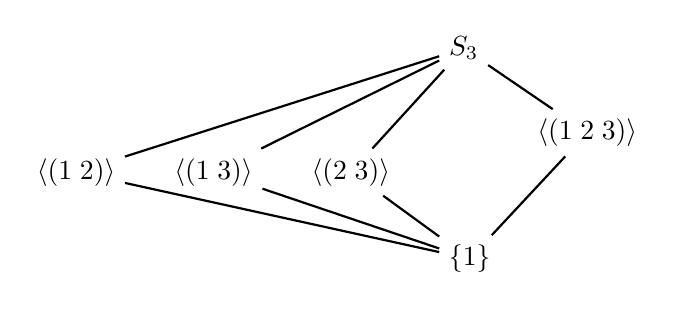
\begin{tikzpicture}[scale=2.5]
        
                \def\d{.5cm}
        
                % Specifies where the x, y coordinate of the tip of
                % the unite vectors in turn
                \tikzset{}
                
                % Scope used to shift the coordinates from the basis
                \begin{scope}[shift={(0, 0, 0)}, rotate=0]
                    \node (S3) at (0, 0) {$S_3$};   
                    \node (A1) [below right=\d and \d of S3]
                    {$\langle (1\;2\;3) \rangle$}; 
                    \node (B1) [below left= 2 * \d and \d of S3]
                    {$\langle (2\;3) \rangle$}; 
                    \node (B2) [left= \d of B1]
                    {$\langle (1\;3) \rangle$};  
                    \node (B3) [left= \d of B2]
                    {$\langle (1\;2) \rangle$};  

                    \node (T1) [below right=\d and \d of B1]
                    {$\left\{ 1 \right\}$}; 
                \end{scope}
        
                \begin{scope}[thick]
                    \draw (S3) -- (A1);
                    \draw (S3) -- (B1);
                    \draw (S3) -- (B2);
                    \draw (S3) -- (B3);
                    \draw (A1) -- (T1);
                    \draw (B1) -- (T1);
                    \draw (B2) -- (T1);
                    \draw (B3) -- (T1);
                \end{scope} 
        
                \end{tikzpicture}
        
                \caption{\label{fig:figure1} Lattice of $S_3.$}
            \end{figure} 

            $C_{S_3}(\{1\}) = S_3$, \\
            $C_{S_3}(\{(1\;2)\}) = \langle (1\;2) \rangle$, \\
            $C_{S_3}(\{(1\;3)\}) = \langle (1\;3) \rangle$, \\
            $C_{S_3}(\{(2\;3)\}) = \langle (2\;3) \rangle$, \\
            $C_{S_3}(\{(1\;2\;3)\}) = \langle (1\;2\;3) \rangle$, \\
            $C_{S_3}(\{(1\;3\;2)\}) = \langle (1\;2\;3) \rangle$.

        \item
            For $D_{16}$,
            we already know that $r^4$ commutes with all other elements:

            \begin{figure}[H]
                \centering
                % figure is a tikz drawing
                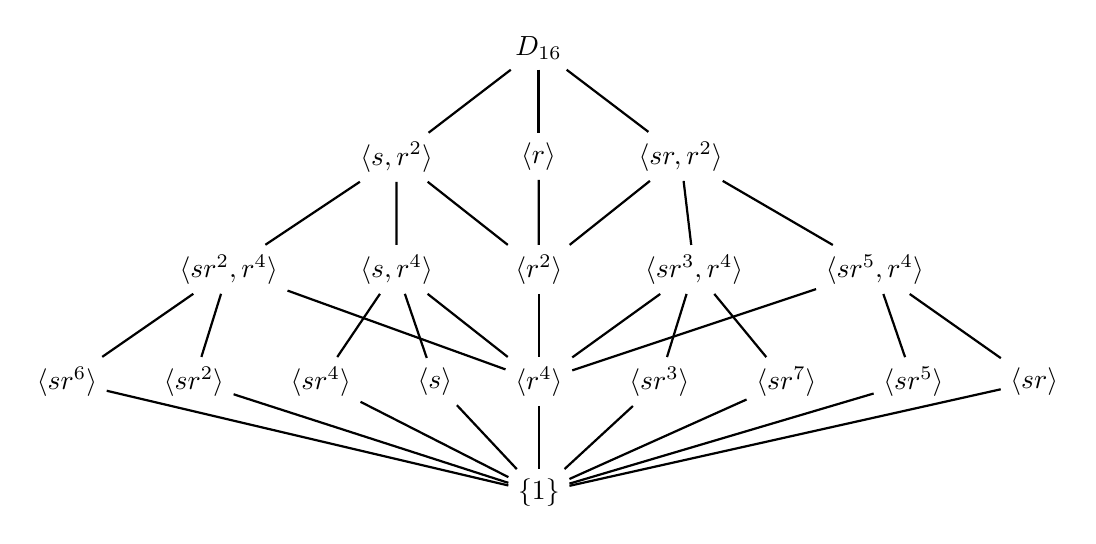
\begin{tikzpicture}[scale=2.5]
        
                \def\d{.8cm}
                \def\h{.6cm}
        
                % Specifies where the x, y coordinate of the tip of
                % the unite vectors in turn
                \tikzset{}
                
                % Scope used to shift the coordinates from the basis
                \begin{scope}[shift={(0, 0, 0)}, rotate=0]
                    \node (D16) at (0, 0) {$D_{16}$};   
                    \node (A1) [below left=\d and \d of D16]
                    {$\langle s, r^2 \rangle$}; 
                    \node (A2) [below= \d of D16] {$\langle r \rangle$}; 
                    \node (A3) [right= \d of A2]
                    {$\langle sr, r^2 \rangle$};  
                    \node (B1) [below left=\d and \d of A1]
                    {$\langle sr^2, r^4 \rangle$}; 
                    \node (B2) [right=\d of B1] {$\langle s, r^4 \rangle$}; 
                    \node (B3) [right=\d of B2]
                    {$\langle r^2 \rangle$};  
                    \node (B4) [right=\d of B3] {$\langle sr^3, r^4 \rangle$}; 
                    \node (B5) [right=\d of B4]
                    {$\langle sr^5, r^4 \rangle$};  
        
                    \node (C1) [below left=\d and \d of B1]
                    {$\langle sr^6 \rangle$}; 
                    \node (C2) [right= \h of C1]
                    {$\langle sr^2 \rangle$}; 
                    \node (C3) [right= \h  of C2]
                    {$\langle sr^4 \rangle$}; 
                    \node (C4) [right= \h of C3]
                    {$\langle s \rangle$}; 
                    \node (C5) [below= \d of B3] {$\langle r^4 \rangle$};
                    \node (C6) [right= \h of C5]
                    {$\langle sr^3 \rangle$}; 
                    \node (C7) [right= \h of C6]
                    {$\langle sr^7 \rangle$};
                    \node (C8) [right= \h of C7]
                    {$\langle sr^5 \rangle$};  
                    \node (C9) [right= \h of C8]
                    {$\langle sr \rangle$};  
                    
                    \node (T1) [below=\d of C5] {$\left\{ 1 \right\}$}; 
                \end{scope}
        
                \begin{scope}[thick]
                    \draw (D16) -- (A1);
                    \draw (D16) -- (A2);
                    \draw (D16) -- (A3);
                    \draw (A1) -- (B1);
                    \draw (A1) -- (B2);
                    \draw (A1) -- (B3);
                    \draw (A3) -- (B5);
                    \draw (A3) -- (B4);
                    \draw (A3) -- (B3);
                    \draw (A2) -- (B3);
                    \draw (B3) -- (C5);
                    \draw (B1) -- (C1);
                    \draw (B1) -- (C2);
                    \draw (B1) -- (C5);
                    \draw (B2) -- (C3);
                    \draw (B2) -- (C4);
                    \draw (B2) -- (C5);
                    \draw (B4) -- (C6);
                    \draw (B4) -- (C7);
                    \draw (B4) -- (C5);
                    \draw (B5) -- (C8);
                    \draw (B5) -- (C9);
                    \draw (B5) -- (C5);
        
                    \foreach\x in {1,..., 9}
                    \draw (C\x) -- (T1);
                \end{scope} 
        
                \end{tikzpicture}
        
                \caption{\label{fig:figure1} Lattice of $D_{16}$.}
            \end{figure} 
                
            $C_{D_{16}}(\{1\}) = D_{16}$, \\
            $C_{D_{16}}(\{r\}) = \langle r \rangle$, \\
            $C_{D_{16}}(\{r^2\}) = \langle r \rangle$, \\
            $C_{D_{16}}(\{r^3\}) = \langle r \rangle$, \\
            $C_{D_{16}}(\{r^4\}) = D_{16}$, \\
            $C_{D_{16}}(\{r^5\}) = \langle r \rangle$, \\
            $C_{D_{16}}(\{r^6\}) = \langle r \rangle$, \\
            $C_{D_{16}}(\{r^7\}) = \langle r \rangle$, \\
            $C_{D_{16}}(\{s\}) = \langle s, r^4 \rangle$, \\
            $C_{D_{16}}(\{sr\}) = \langle r^4, sr^5 \rangle$, \\
            $C_{D_{16}}(\{sr^2\}) = \langle r^4, sr^2 \rangle$, \\
            $C_{D_{16}}(\{sr^3\}) = \langle r^4, sr^2 \rangle$, \\
            $C_{D_{16}}(\{sr^4\}) = \langle s, r^4 \rangle$, \\
            $C_{D_{16}}(\{sr^5\}) = \langle r^4, sr^5 \rangle$, \\
            $C_{D_{16}}(\{sr^6\}) = \langle r^4, sr^2 \rangle$, \\
            $C_{D_{16}}(\{sr^7\}) = \langle r^4, sr^3 \rangle$.  
    \end{enumerate}


    \section*{Exercise 7}
    The center of $D_{16}$ is the set of elements 
    that commute with all others in the group.
    From exercise 1.2.5.6, we know that the only elements
    such that their centralizer is the entire group $D_{16}$
    are $1$ and $r^4$.
    That makes them the only elements in $D_{16}$ to commute
    with the whole group.
    We can also point to exercise 1.2.2.7,
    where we showed $Z(D_{2n}) = \{1, r^n\}$ if $n$ is even.
    So $Z(D_{16}) = \{1, r^4\}$.


    \section*{Exercise 8}
    We know that the normalizers of each group are a subgroup
    of that group,
    so they will feature in its lattice.
    So we will check for each subgroup whether or not it commutes
    set wise with each of the group's subgroups
    to determine the highest subgroup that commutes with it.
    We choose the highest subgroup because the normalizer
    is the set of all elements that have these properties:
    \begin{enumerate}[label=\textbf{\alph*.}]
        \item
            For $S_3$,
            Every subgroup except for the trivial one is maximal,
            and every subgroup is cyclic,
            so every subgroup is contained in its own normalizer.
            That means that for $H \seq S_3$,
            $N_{S_3}(H) = H$ or $S_3$:

            \begin{figure}[H]
                \centering
                % figure is a tikz drawing
                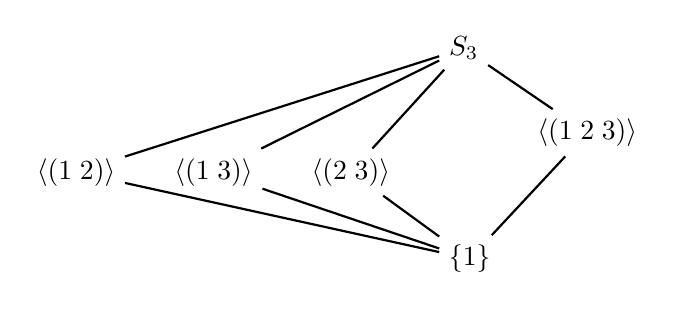
\begin{tikzpicture}[scale=2.5]

                \def\d{.5cm}

                % Specifies where the x, y coordinate of the tip of
                % the unite vectors in turn
                \tikzset{}
                
                % Scope used to shift the coordinates from the basis
                \begin{scope}[shift={(0, 0, 0)}, rotate=0]
                    \node (S3) at (0, 0) {$S_3$};   
                    \node (A1) [below right=\d and \d of S3]
                    {$\langle (1\;2\;3) \rangle$}; 
                    \node (B1) [below left= 2 * \d and \d of S3]
                    {$\langle (2\;3) \rangle$}; 
                    \node (B2) [left= \d of B1]
                    {$\langle (1\;3) \rangle$};  
                    \node (B3) [left= \d of B2]
                    {$\langle (1\;2) \rangle$};  

                    \node (T1) [below right=\d and \d of B1]
                    {$\left\{ 1 \right\}$}; 
                \end{scope}

                \begin{scope}[thick]
                    \draw (S3) -- (A1);
                    \draw (S3) -- (B1);
                    \draw (S3) -- (B2);
                    \draw (S3) -- (B3);
                    \draw (A1) -- (T1);
                    \draw (B1) -- (T1);
                    \draw (B2) -- (T1);
                    \draw (B3) -- (T1);
                \end{scope} 

                \end{tikzpicture}

                \caption{\label{fig:figure1} Lattice of $S_3$.}
            \end{figure} 

            $N_{S_3}(\{1\}) = S_3$, \\
            $N_{S_3}(\langle (1\;2) \rangle) = \langle (1\;2) \rangle$, \\
            $N_{S_3}(\langle (1\;3) \rangle) = \langle (1\;3) \rangle$, \\
            $N_{S_3}(\langle (2\;3) \rangle) = \langle (2\;3) \rangle$, \\
            $N_{S_3}(\langle (1\;2\;3) \rangle) = S_3$, \\
            $N_{S_3}(S_3) = S_3$.

        \item

            For $Q_8$,
            the 3 subgroups generated by imaginary numbers
            are maximal,
            so they either they or the entire group is their own normalizer:
            
            \begin{figure}[H]
                \centering
                % figure is a tikz drawing
                \begin{tikzpicture}[scale=2.5]

                \def\d{.5cm}

                % Specifies where the x, y coordinate of the tip of
                % the unite vectors in turn
                \tikzset{}
                
                % Scope used to shift the coordinates from the basis
                \begin{scope}[shift={(0, 0, 0)}, rotate=0]
                    \node (Q8) at (0, 0) {$Q_8$};   
                    \node (A1) [below left=\d and \d of G1]
                    {$\langle i \rangle$}; 
                    \node (A2) [below= \d of G1] {$\langle j \rangle$}; 
                    \node (A3) [below right=\d and \d of G1]
                    {$\langle k \rangle$};  
                    \node (B3) [below= \d of A2]
                    {$\langle -1 \rangle$};  
                    \node (T1) [below=\d of B3] {$\left\{ 1 \right\}$}; 
                \end{scope}

                \begin{scope}[thick]
                    \draw (Q8) -- (A1);
                    \draw (Q8) -- (A2);
                    \draw (Q8) -- (A3);
                    \draw (A1) -- (B3);
                    \draw (A3) -- (B3);
                    \draw (A2) -- (B3);
                    \draw (B3) -- (T1);
                \end{scope} 

                \end{tikzpicture}
            \caption{\label{fig:figure1} Lattice of $Q_8.$}
            \end{figure} 

            $N_{Q_8}(\{1\}) = Q_8$, \\
            $N_{Q_8}(\langle i \rangle) = Q_8$, \\
            $N_{Q_8}(\langle j \rangle) = Q_8$, \\
            $N_{Q_8}(\langle k \rangle) = Q_8$, \\
            $N_{Q_8}(\langle -1 \rangle) = Q_8$, \\
            $N_{Q_8}(Q_8) = Q_8$.
    \end{enumerate}


    \section*{Exercise 9}
    Referring to exercise 1.2.3.6,
    we know all the subgroups and inclusions
    of $\Z/48\Z$ (same applies for $\Z/16\Z$ and $\Z/24\Z$):
    \begin{enumerate}[label=\textbf{\alph*.}]
        \item
            For $\Z/16\Z$:

            \begin{figure}[H]
                \centering
                % figure is a tikz drawing
                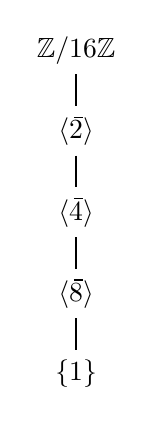
\begin{tikzpicture}[scale=2.5]

                \def\d{.4cm}

                % Specifies where the x, y coordinate of the tip of
                % the unite vectors in turn
                \tikzset{}
                
                % Scope used to shift the coordinates from the basis
                \begin{scope}[shift={(0, 0, 0)}, rotate=0]

                    \node (1) at (0, 0)
                    {$\Z/16\Z$}; 
                    \node (2) [below=\d of 1]
                    {$\langle \olsi{2} \rangle$}; 
                    \node (4) [below= \d of 2]
                    {$\langle \olsi{4} \rangle$}; 
                    \node (8) [below= \d of 4]
                    {$\langle \olsi{8} \rangle$};
                    \node (0) [below= \d of 8]
                    {$\{1\}$}; 
                \end{scope}

                \begin{scope}[thick]
                    \draw (1) -- (2);
                    \draw (2) -- (4);
                    \draw (4) -- (8);
                    \draw (8) -- (0);
                \end{scope} 

                \end{tikzpicture}
            \caption{\label{fig:figure1} Lattice of $\Z/16\Z$.}
            \end{figure} 
        \item
            For $\Z/24\Z$:

            \begin{figure}[H]
                \centering
                % figure is a tikz drawing
                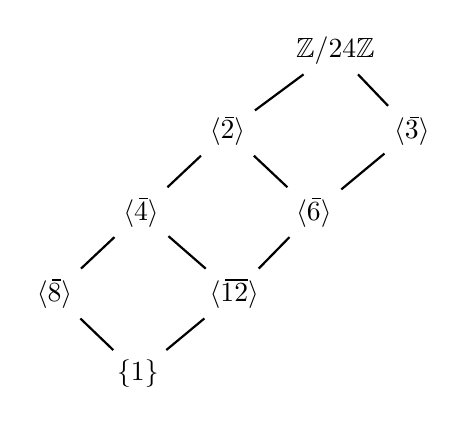
\begin{tikzpicture}[scale=2.5]

                \def\d{.4cm}
                \def\v{0cm}

                % Specifies where the x, y coordinate of the tip of
                % the unite vectors in turn
                \tikzset{}
                
                % Scope used to shift the coordinates from the basis
                \begin{scope}[shift={(0, 0, 0)}, rotate=0]

                    \node (1) at (0, 0) {$\Z/24\Z$}; 
                    \node (2) [below left=\d and \d of 1]
                    {$\langle \olsi{2} \rangle$}; 
                    \node (3) [below right=\d and \v of 1]
                    {$\langle \olsi{3} \rangle$}; 
                    \node (4) [below left=\d and \d of 2]
                    {$\langle \olsi{4} \rangle$}; 
                    \node (6) [below right=\d and \d of 2]
                    {$\langle \olsi{6} \rangle$}; 
                    \node (8) [below left=\d and \d of 4]
                    {$\langle \olsi{8} \rangle$}; 
                    \node (12) [below right=\d and \d of 4]
                    {$\langle \olsi{12} \rangle$}; 
                    \node (0) [below left=\d and \d of 12]
                    {$\{1\}$}; 
                \end{scope}

                \begin{scope}[thick]
                    \draw (1) -- (2);
                    \draw (1) -- (3);
                    \draw (2) -- (4);
                    \draw (2) -- (6);
                    \draw (4) -- (8);
                    \draw (4) -- (12);
                    \draw (3) -- (6);
                    \draw (6) -- (12);
                    \draw (8) -- (0);
                    \draw (12) -- (0);
                \end{scope} 

                \end{tikzpicture}
            \caption{\label{fig:figure1} Lattice of $\Z/24\Z$.}
            \end{figure} 
        \item
            For $\Z/48\Z$:

            \begin{figure}[H]
                \centering
                % figure is a tikz drawing
                \begin{tikzpicture}[scale=2.5]

                \def\d{.4cm}
                \def\v{0cm}

                % Specifies where the x, y coordinate of the tip of
                % the unite vectors in turn
                \tikzset{}
                
                % Scope used to shift the coordinates from the basis
                \begin{scope}[shift={(0, 0, 0)}, rotate=0]

                    \node (1) at (0, 0) {$\Z/48\Z$}; 
                    \node (2) [below left=\d and \d of 1]
                    {$\langle \olsi{2} \rangle$}; 
                    \node (3) [below right=\d and \v of 1]
                    {$\langle \olsi{3} \rangle$}; 
                    \node (4) [below left=\d and \d of 2]
                    {$\langle \olsi{4} \rangle$}; 
                    \node (6) [below right=\d and \d of 2]
                    {$\langle \olsi{6} \rangle$}; 
                    \node (8) [below left=\d and \d of 4]
                    {$\langle \olsi{8} \rangle$}; 
                    \node (12) [below right=\d and \d of 4]
                    {$\langle \olsi{12} \rangle$}; 
                    \node (16) [below left=\d and \d of 8]
                    {$\langle \olsi{16} \rangle$}; 
                    \node (24) [below right=\d and \d of 8]
                    {$\langle \olsi{24} \rangle$};  
                    \node (0) [below left=\d and \d of 24]
                    {$\{1\}$}; 
                \end{scope}

                \begin{scope}[thick]
                    \draw (1) -- (2);
                    \draw (1) -- (3);
                    \draw (2) -- (4);
                    \draw (2) -- (6);
                    \draw (4) -- (8);
                    \draw (4) -- (12);
                    \draw (8) -- (16);
                    \draw (8) -- (24);
                    \draw (16) -- (0);
                    \draw (3) -- (6);
                    \draw (6) -- (12);
                    \draw (12) -- (24);
                    \draw (24) -- (0);
                \end{scope} 

                \end{tikzpicture}
            \caption{\label{fig:figure1} Lattice of $\Z/48\Z$.}
            \end{figure} 
    \end{enumerate}


    \section*{Exercise 10 $***$}
    Proof that if $|G| = 4$, 
    then $G \cong Z_4$ (cyclic group) or $G \cong V_4$ (Klein group): \\
    We know from our proof in exercise 1.1.1.36 that a group
    of order 4 where none of the elements have order 4
    is unique and has the following table:
    \begin{figure}[H]
        \centering

        \[\vbox{\tabskip0.5em\offinterlineskip
        \halign{\strut$#$\hfil\ \tabskip1em\vrule&&$#$\hfil\cr
        ~   & 1   & a   & b & c \cr
        \noalign{\hrule}\vrule height 12pt width 0pt
        1   & 1 & a & b & c \cr 
        a   & a & 1 & c & b \cr 
        b   & b & c & 1 & a \cr 
        c   & c & b & a & 1 \cr
        }}\]

        \caption{\label{fig:figure1} The table of the described group.}
    \end{figure}
    
    This is obviously the group table of the Klein group,
    so every group of order 4 that doesn't have
    an element with order 4 is unique and isomorphic to $V_4$. \\
    To add to the prood, if $|G| = 4$ and there exists
    an element $x \in G$ with order 4 as well,
    then by exercise 1.1.1.32, since $|x| = 4$,
    $1, x, x^2, x^3$ are all unique elements.
    Since $G$ is closed under multiplication,
    all 4 elements are in $G$.
    And since $G = 4$, then $G = \{1, x, x^2, x^3\}$.
<<<<<<< HEAD
    So $G = Z_4$.
    So any group of order 4 where one element has order 4 as well
    must be isomorphic to $Z_4$.


    \section*{Exercise 11 $***$}
    Let
    \[ QD_{16} = \langle \sigma, \tau \mid \sigma^8 = \tau^2 = 1,
    \sigma\tau = \tau\sigma^3 \rangle \] 
    Be a group of order 16
    (called the \textit{Quasidihedral} or \textit{Semidihedral
    Group of order 16}).
    This group has 3 subgroups of order 8,
    which are
    \[ \langle \tau, \sigma^2 \rangle \cong D_8, \qquad
    \langle \sigma \rangle \cong Z_8, \qquad
    \langle \sigma^2, \tau\sigma \rangle \cong Q_8 \]
    Every proper subgroup of $QD_{16}$ is contained inside one of those
    3 subgroups.
    To complete the given lattice of $QD_{16}$ by filling in the missing
    subgroups using at most two generators,
    we can use the lattices of $D_8$, $Z_8$ and $Q_8$
    in order to help us,
    since isomorphic groups have the same lattices. \\
    According to exercise 1.1.5.3,
    $Q_8$ is generated by $i$ and $j$,
    so $\langle i, j \rangle \cong \langle \sigma^2, \tau\sigma \rangle$.
    We know that $Q_8$ has 3 maximal subgroups,
    $\langle i \rangle$, $\langle j \rangle$, and $\langle k \rangle$,
    all of which are cyclic.
    This means that in $QD_{16}$,
    $\langle \sigma^2, \tau\sigma \rangle$
    will have 3 subgroups,
    $\langle \sigma^2 \rangle$,
    $\langle \tau\sigma \rangle$
    and 
    $\langle \sigma^2\tau\sigma \rangle$
    (since $ij = k$).
    The leftmost subgroup is supposed to be $\langle \sigma^2 \rangle$
    because it's contained inside $\langle \sigma \rangle$,
    which is cyclic and only contains cyclic subgroups generated
    by a power of $\sigma$.
    The order of the other two doesn't matter. \\
    Now if we look at the lattice of $D_8$,
    we note that it also has 3 maximal subgroups,
    which are $\langle r \rangle$,
    $\langle s, r^2 \rangle$, 
    and $\langle rs, r^2 \rangle$.
    We know that
    $D_8 = \langle r, s \rangle \cong \langle \sigma^2, \tau \rangle$,
    so if we map $r$ to $\sigma^2$ and $s$ to $\tau$,
    we see that in the $QD_{16}$ lattice,
    $\langle \sigma^2, \tau \rangle$
    already contains $\langle \sigma^2\rangle$, or $\langle r \rangle$,
    and $\langle \sigma^4, \tau \rangle$, or $\langle r^2, s \rangle$.
    This leaves $\langle rs, r^2  \rangle$,
    which in this case is the leftmost subgroup
    $\langle \sigma^2\tau, \sigma^4 \rangle$. \\
    Now in $D_8$,
    the subgroup $\langle r^2, s  \rangle$
    also contains 3 subgroups,
    which are $\langle r^2 \rangle$,
    $\langle s \rangle$,
    and $\langle r^2s \rangle$,
    which correspond to
    $\langle \sigma^4 \rangle$,
    $\langle \tau \rangle$,
    and $\langle \sigma^4\tau \rangle$.
    These will be the subgroups of
    $\langle \sigma^4, \tau \rangle$ in the lattice.
    The first two of the subgroups already exist,
    so we add the third. \\
    Also in $D_8$ is the subgroup $\langle rs, r^2  \rangle$
    also contains 3 subgroups,
    which are $\langle r^2 \rangle$,
    $\langle rs \rangle$,
    and $\langle r^3s \rangle$,
    which correspond to
    $\langle \sigma^4 \rangle$,
    $\langle \sigma^2\tau \rangle$,
    and $\langle \sigma^6\tau \rangle$.
    These will be the subgroups of
    $\langle \sigma^2\tau, \sigma^4 \rangle$ in the lattice.
    The first and third the subgroups already exist.
    This is because, for the third subgroup,
    $\sigma^6\tau = \sigma^{5}\sigma\tau = \sigma^5\tau\sigma^3 = \dots
    = \tau\sigma^{18} = \tau\sigma^{16}\sigma^2
    = \tau(\sigma^{8})^2\sigma^2 = \tau\sigma^2$.
    So we add the second subgroup $\langle \sigma^2\tau \rangle$
    to the lattice.

    \begin{figure}[H]
        \centering
        % figure is a tikz drawing
        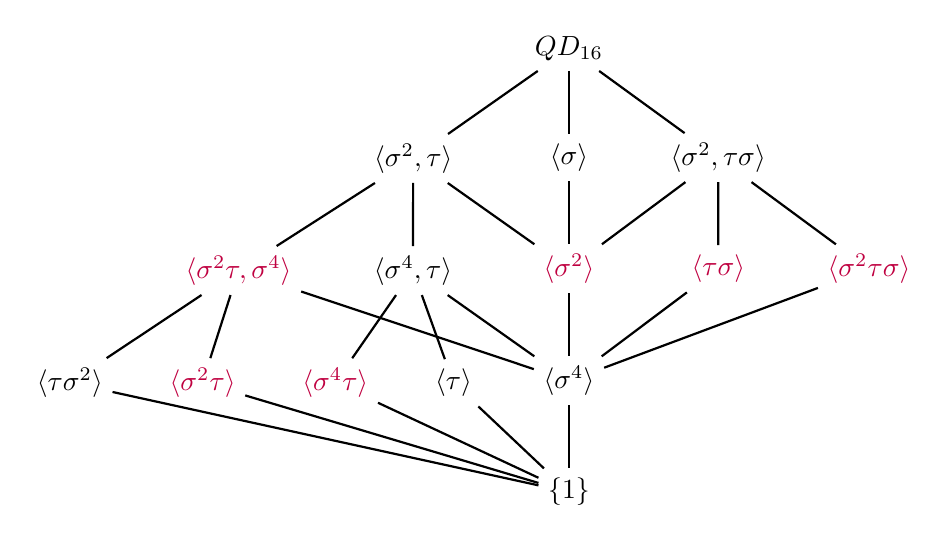
\begin{tikzpicture}[scale=2.5]

        \def\d{.8cm}
        \def\h{.6cm}

        % Specifies where the x, y coordinate of the tip of
        % the unite vectors in turn
        \tikzset{}
        
        % Scope used to shift the coordinates from the basis
        \begin{scope}[shift={(0, 0, 0)}, rotate=0]
            \node (D16) at (0, 0) {$QD_{16}$};   
            \node (A1) [below left=\d and \d of D16]
            {$\langle \sigma^2, \tau \rangle$}; 
            \node (A2) [below= \d of D16] {$\langle \sigma \rangle$}; 
            \node (A3) [right= \d of A2]
            {$\langle \sigma^2, \tau\sigma \rangle$};  
            \node (B1) [below left=\d and \d of A1]
            {\textcolor{purple}{$\langle \sigma^2\tau, \sigma^4 \rangle$}}; 
            \node (B2) [right=\d of B1] {$\langle \sigma^4, \tau \rangle$}; 
            \node (B3) [below=\d of A2]
            {\textcolor{purple}{$\langle \sigma^2 \rangle$}};  
            \node (B4) [below=\d of A3]
            {\textcolor{purple}{$\langle \tau\sigma \rangle$}}; 
            \node (B5) [right=\d of B4]
            {\textcolor{purple}{$\langle \sigma^2\tau\sigma \rangle$}};  

            \node (C1) [below left=\d and \d of B1]
            {$\langle \tau\sigma^2 \rangle$}; 
            \node (C2) [right= \h of C1]
            {\textcolor{purple}{$\langle \sigma^2\tau \rangle$}}; 
            \node (C3) [right= \h  of C2]
            {\textcolor{purple}{$\langle \sigma^4\tau \rangle$}}; 
            \node (C4) [right= \h of C3]
            {$\langle \tau \rangle$}; 
            \node (C5) [below= \d of B3] {$\langle \sigma^4 \rangle$};

            
            \node (T1) [below=\d of C5] {$\left\{ 1 \right\}$}; 
        \end{scope}

        \begin{scope}[thick]
            \draw (D16) -- (A1);
            \draw (D16) -- (A2);
            \draw (D16) -- (A3);
            \draw (A1) -- (B1);
            \draw (A1) -- (B2);
            \draw (A1) -- (B3);
            \draw (A3) -- (B5);
            \draw (A3) -- (B4);
            \draw (A3) -- (B3);
            \draw (A2) -- (B3);
            \draw (B3) -- (C5);
            \draw (B1) -- (C1);
            \draw (B1) -- (C2);
            \draw (B1) -- (C5);
            \draw (B2) -- (C3);
            \draw (B2) -- (C4);
            \draw (B2) -- (C5);
            \draw (B4) -- (C5);
            \draw (B5) -- (C5);

            \foreach\x in {1,..., 5}
            \draw (C\x) -- (T1);
        \end{scope} 

        \end{tikzpicture}

        \caption{\label{fig:figure1} Lattice of $QD_{16}$.}
    \end{figure} 


    \section*{Exercise 12}
%     \begin{tikzpicture}[
%         declare function = {
%             Z(\x,\y) = e^(-(\x^2 + \y^2));
%         }
%     ]
%     \begin{axis}
%     [
%     axis lines=center,
%     unit vector ratio=1 1 1, % or axis equal, which dsiables scaling
%     enlargelimits,
%     tick align=inside,
%     domain=-3:3,
%     samples=30, % number of panels
%     minor tick num=5,
%     ]
%     \addplot3 [surf] {Z(x,y)};
%     \end{axis}
% \end{tikzpicture}


=======
    So $G = \Z_4$.
    So any group of order 4 where one element has order 4 as well
    must be isomorphic to $Z_4$.

>>>>>>> c733b4c556979a7348397865067ed20806b6465e
\end{document}
